\documentclass[11pt,a4paper]{article}
\usepackage[utf8]{inputenc}
\usepackage[dutch]{babel}
\usepackage{amsmath}
\usepackage{amsfonts}
\usepackage{amssymb}
\usepackage{graphicx}
\usepackage{pdfpages}

\author{Pieter Van Keymeulen}
\title{NonkelScript}

\begin{document}

\includepdf{afbeeldingen/voorblad}
\newpage

\tableofcontents
\newpage

\section{Introductie}
Bedrijven zijn er in alle soorten en maten. Niet ieder bedrijf heeft dezelfde specialisatie en iedere onderneming verkoopt andere diensten naargelang hun aard. Neem nu een horecabedrijf in vergelijking met een supermarkt. Een restaurant heeft een variabel aanbod. Het menu kan van dag tot dag wisselen, evenals de prijzen die zelfs kunnen variëren van uur tot uur. Een supermarkt daarentegen heeft een vast aantal producten en de prijzen van deze producten variëren niet zo vaak.

Bij het maken van een ERP systeem is het belangrijk dat we kunnen inspelen op de noden van de klant. We kunnen een ERP systeem zodanig maken dat de klant dit door middel van scripts kan aanpassen. In ons geval spreken we van scripts die de klant in staat stellen fouten die gebeuren binnen het systeem op te vangen. Dit kan gaan van simpele dingen zoals een printer die zonder inkt komt te liggen, tot meer complexe omstandigheden zoals het blokkeren van de productie van goederen. In beide gevallen moet er een soort fout gegenereerd worden die afgevangen kan worden. De klant zal deze fout op zijn eigen manier willen afhandelen. Door middel van onze scripttaal is dat van nu af aan mogelijk.

Nonkelscript is een scriptingtaal met ingebouwde multithreading. Als de verdere ontwikkelingen het ons toelaten zal de Nonkelscript interpreter in de toekomst kunnen draaien als daemon. Deze daemon zal in staat zijn de verschillende subsystemen van het ERP systeem te ondervragen. Verder zal de daemon enkele scripts toegewezen krijgen die gekoppeld kunnen worden aan een bepaalde fout die het ERP systeem kan genereren.

\section{Over programmeertalen}
\subsection{Geschiedenis}
%notities over deze sectie.
%Zorgen dat ik zo weinig mogelijk namen noem en, indien ik dit wel doe, ze eerst goed opzoek
%Evoor zorgen dat de aanhalingstekens goed getoond worden
Al vanaf het levenslicht van de eerste computer (De Z1 van Konrad Zuse) bestond er de nood om deze geweldige machines te programmeren. Computers moesten in staat zijn om een door de mens neergeschreven opdracht te kunnen uitvoeren. Dit konden hele complexe taken zijn. Van een simpele optelling tot het sorteren van een volledige reeks getallen. Een eerste poging tot het maken van zo een machine werd gedaan door Charles Babage. Het ontwerp van deze machine bleek echter te complex om ooit uitgevoerd te worden. Babbage had namelijk er geen rekening mee gehouden dat het arabische telsysteem veel complexer is dan het op het eerste gezicht lijkt. Dat bestaat namelijk uit 10 cijfers. Wat redelijk complex is om te implementeren gezien dat ieder cijfer voorgesteld moet worden. Dat betekent dat men 10 "states" nodig heeft om getallen te kunnen uitdrukken. Hoe moet dit uitgedrukt worden. Konrad Zuse had dit opgelost door het binaire systeem te gebruiken. Hierbij waren er slechts twee "states" nodig. Namelijk "waar" of "vals"

\subsection{Waarom niet één programmeertaal?}
Niet alles is even belangrijk op ieder werkveld. In de industrie is het vooral de veiligheid belangrijk. Stel dat er tijdens het productieproces bijvoorbeeld een fout zou gebeuren en dat het corrigeren van deze fout van groot belang is. Dan is het wenselijk dat de programma's die verantwoordelijk zijn voor het corrigeren van deze fout ook zo snel mogelijk kunnen reageren. Om dit te bereiken moet de gebruikte programmeertaal zo laag mogelijk zijn. Dit wil zeggen, zo dicht mogelijk aanliggen bij de eigenlijke werking van de machine. Dit laat de programmeur toe om enorm veel details van het programma te controleren.

Omgekeerd is ook mogelijk. het programmeren in assembler kan namelijk erg tijdrovend zijn. Zeker wanneer de te programmeren programma's ingewikkelder worden. Het is erg moeilijk een grafisch programma (maar niet onmogelijk) te maken met assembler. Ook omdat assembler een ongestructureerde programmeertaal is (meer hierover straks) en daarom de kans groot dat je uitkomt in zogenaamde "spaghetticode". Deze code wordt na verloop van tijd onhandelbaar. Het is dan wenselijk enige abstractie in de code te brengen. Dit kan door middel van in eerste instantie objectgeoriënteerd programmeren en, in tweede instantie proceduraal programmeren. Beide manier worden later in het verslag uitvoerig besproken.

\subsection{Waarom nog een nieuwe programmeertaal maken?}
Het maken van een nieuwe programmeertaal brengt vele voordelen met zich mee. Er zijn namelijk weinig echt pure multi purpose talen terwijl dat er veel gespecialiseerde talen zijn. Dit heeft zo zijn redenen. Het maken van een eigen programmeertaal leent zich namelijk tot het perfect aanpassen van deze programmeertaal. Neem nu een voorbeeld aan ADA. Dit is een programmeertaal die speciaal gemaakt is voor militaire doeleinden. Het heeft de volgende features.

\begin{description}
\item[Sterke typering] Objecten van het éne type kunnen niet zomaar geconverteerd worden naar objecten van het andere type.
\item[Modulariteit] Het is in ADA mogelijk om zogenaamde packages te maken zodat een programma opgesplitst kan worden in meerdere bestanden.
\item[Run-time checking] Een aan de standaard houdende ADA compiler moet de mogelijkheid bieden om zogenaamde run-time checks uit te voeren. Deze kijken na over geen typecast fouten, stack overflows, wiskundige fouten etc \ldots in het programma bevinden.
\item[Exceptie handeling] Het is in ADA mogelijk om verschillende fouten af te handelen die naar de programmeur gegooid worden. Hoewel hetzelfde effect ook bereikt kan worden is leuk dat we door hier een speciale syntaxis te voorzien we hier speciale features aan kunnen toevoegen zodat de code beter leesbaar wordt en er minder variabelen nodig zijn voor het afhandelen van fouten.
\end{description}

\section{ERP systemen}

%vertel hier over de api van NonkelErp

\section{Bison en flex}
Bison en Flex zijn twee programma's die tezamen gebruikt kunnen worden voor het maken van een compiler. Met Flex kan er via reguliere expressies een "tokenizer" gemaakt worden die gebruikt kan worden om broncode te scannen op bepaalde sleutelwoorden. De informatie de Flex op deze manier verzameld kan op zijn beurt weer gebruikt worden door Bison. Deze vraagt de gescande sleutelwoorden kunnen gebruikt worden voor het opstellen van regels geschreven in Bakkus-Naur vorm. Aan iedere regel kan er een actie gekoppeld worden. Dit is een stuk code. Meestal is deze code geschreven in C, maar aangezien onze compiler in Delphi geschreven zal worden zal deze code dan ook Delphi zijn. De parser die uit deze verzameling regels gegenereerd zal worden zal naar iedere regel zoeken telkens wanneer er één van die regels gevonden wordt de gekoppelde actie uitvoeren. Op deze manier kan er op een efficiënte wijze een interpeter gemaakt worden.

\subsection{Flex}
Zoals eerder gezegd werkt flex door middel van reguliere expressies. Deze expressies kunnen net zoals in Bison gekoppeld worden aan een actie. Deze actie wordt net zoals in de Bison parser uitgevoerd. In een standaard Flex scanner doen deze acties niet zoveel. Eigenlijk geven ze gewoon tokens terug die correspondeert met de gevonden reguliere expressie. 

\subsection{Bison}
Bison is ongeveer hetzelfde als flex. Met het verschil dat bison de informatie van die flex doorgeeft opvangt, verwerkt, en vergelijkt met een aantal regels. De regels worden geschreven in bakkus-naur vorm. Ook deze regels zijn gekoppeld aan een actie die uitgevoerd wordt wanneer de regel in de broncode gevonden wordt.

In ons geval gaan we voor iedere gevonden regel een node maken en deze node in onze syntaxboom stoppen. Meer hierover straks.

\section{Interne structuur van de compiler}
Voor het programmeren van de compiler werd er gekozen voor Delphi. Wat niet een voor de hand liggende keuze is. Zowel Bison als Flex zijn immers beiden ontworpen om gebruikt te worden in combinatie met C. De reden voor deze vreemde keuze is dat de compiler moet kunnen integreren met een bestaand ERP systeem en dit systeem is geschreven in Delphi. Freepascal (de compiler die we gebruiken voor het bouwen van onze compiler) komt echter gebundeld met een programma dat in staat is om Bison en Flex code te converteren naar een Pascal unit. Hoewel deze tool is gemaakt in 2001 en eigenlijk bedoeld is voor gebruik in combinatie met Turbo Pascal volstaat het voor ons doel.

\subsection{broncode naar programma}

\subsubsection{Front end}
Zowel Flex als Bison zijn zogenaamde parsergenerators. Dit wil zeggen dat zij een formele grammatica aanvaarden. Deze formele grammatica is meestal opgeschreven in Bakus-Naur vorm. Nadat de parsergenerator de grammatica heeft verwerkt genereert deze een parser in een bepaalde doelprogrammeertaal. Dit kan in C, C++, Pascal en dergelijke zijn. Deze parser kan daarna als component in de compiler gebruikt worden en helpt bij het scannen en analyseren van de broncode.

Buiten het parsen van de broncode, is de front-end verantwoordelijk voor nog een aantal taken. De belangrijkste hiervan is het omzetten van de broncode naar een interne representatie. Dit is een abstracte representatie van broncode ontdaan van alles wat niet relevant is voor het interpreteren van het programma. De manier waarop dit intern gerepresenteerd moet worden is vrij. De meestgebruikte technieken zijn een syntaxboom en een lineaire representatie. 

\subsubsection{back end}
Hoewel dit onderdeel niet altijd aanwezig is in iedere compiler, voert dit gedeelte, indien aanwezig, nodige extra optimalisaties uit. Naast dit voeren sommige compiler ook nog een verdere analyse uit op de abstract syntax tree.

Tijdens deze analyse wordt er aandacht besteed aan twee onderdelen van de code. Namelijk de data flow en de control flow. Het doel echter van deze analyse blijft het optimaliseren van de code. Hiermee bedoelen we iedere bewerking op de code die het programma sneller zal doen draaien terwijl het hetzelfde resultaat levert. Met optimalisaties moet men heel voorzichtig omspringen, omdat men nooit de daadwerkelijke bedoelingen van de programmeur weet.


\begin{description}
\item[Dode code] Soms heeft een programma zogenaamde dode code. Dit is code die wel mee in het uiteindelijke uitvoerbare programma zit, maar die eigenlijk nooit wordt uitgevoerd. In zulke gevallen kunnen we de snelheid van het programma vergroten door deze code gewoon weg te laten. Hetzelfde voorbeeld kan nog veel verder getrokken worden. Stel dat men als debugger een programma aan het maken is en men wilt bepaalde code testen. Dan wordt vaak, ookal is dat niet echt aan te raden, een aparte functie gemaakt die het te testen object als parameter meekrijgt. Dit louter om het object naar de terminal te schrijven zodat de inhoud ervan door de ontwikkelaar gelezen kan worden. Naargelang het productieproces vordert worden de aanroepen van deze functies verwijderd, waardoor deze code niet meer wordt uitgevoerd en eigenlijk overbodig is.

\begin{verbatim}
if (n >= 0) {
  // n groter of gelijk aan 0
} else if (n < 0) {
  // n kleiner dan 0
} else {
  // dood
}
\end{verbatim}

Dit soort code heeft enkele grote nadelen.
\begin{itemize}
\item Bij het ontwikkelen wordt er vaak veel tijd verspild aan dode code.
\item Dode code verspilt geheugen aangezien deze code toch niet gebruikt wordt.
\end{itemize}

\item[Redundante code] Redundante code is zo ongeveer hetzelfde als gewone code, met het verschil dat de code wel uitgevoerd wordt, maar er eigenlijk niets mee wordt gedaan. Dit kan een berekening zijn of de uitvoer van een functie. Ook hier is het, indien dit geen invloed heeft op de uitvoer van het programma, het beste dat we deze code weglaten.

\begin{verbatim}
const char * a = "redundante variable";
const char* b = "niet redundante variable;

printf("%s", b);
\end{verbatim}

\end{description}

%\subsubsection{back end}
%Hier komt de tekst over de back end

\subsection{variabelesystemen}
\subsubsection{Variabelen}
Een programma maakt berekeningen. Het spreekt voor zich dat deze berekeningen moeten kunnen worden opgeslagen zodat het mogelijk is om het resultaat van de berekening te gebruiken in een andere berekening. Men moet hier echter bij bedenken dat er verschillende manieren bestaan om dit binnen een programmeertaal aan te pakken. Intuïtief zou men dit kunnen doen.

\begin{verbatim}
a:= 7;
b:= 10.27;
c:= a + b;
\end{verbatim}

Als men deze code zou bekijken zou men kunnen denken dat dit de makkelijkste manier is om dit op te schrijven. Dit komt bijna overeen met hoe een doorsnee mens deze bewerkingen op papier zou schrijven. Dit wordt echter in een programmeertaal niet zo vaak gedaan omdat dit een enorm nadeel heeft voor de compiler. De compiler weet namelijk niet welk type aan de variabele toegekend wordt. Indien de compiler dit wel weet kan de compiler hierop inspelen door exact die hoeveelheid geheugen te reserveren die nodig is voor het opslaan van die variabele. Dit kan op de volgende manier.

\begin{verbatim}
int a:= 7;
int b:= 8;
int c:= a + b;
\end{verbatim}

De eerste methode wordt dynamische typering genoemd. De tweede statische. Het is duidelijk dat, hoewel de tweede methode beter is voor de compiler, de eerste methode vlotter schrijft. Daarom wordt er in een scripttaal vaak gebruik gemaakt van dynamische typering omdat hier vaak de snelheid minder belangrijk is en deze talen voornamelijk bedoeld zijn om snel kleine programma's te kunnen schrijven.  

\section{Design}
Onze compiler is gebaseerd op twee grote design pattern. Het composite design pattern, dat gebruikt wordt om de syntaxboom te bouwen en het interpreter design pattern, dat gebruikt wordt om de interpreter te bouwen. Beide zullen in dit hoofdstuk uitgelegd worden.

Voor het programmeren van systeemapplicaties is statische typering meestal te prefereren boven dynamische. Veel compilers voeren namelijk zogenaamde typechecks uit. Voordat een bepaald stuk code wordt gecompileerd wordt er eerst bekeken, indien dit bijvoorbeeld een toekenning is, of de waarde die toegekend wordt aan de variabele wel degelijk in de variabele kan. Indien niet wordt er een fout gegeneerd. Bij dynamische typering is dit niet mogelijk tijdens het compileren, maar tijdens het uitvoeren van het programma. Dit omdat men nooit weet, bij een dynamisch getypeerde taal, welk type een variabele uiteindelijk gaat hebben. Dit is een nadeel in een omgeving waar snelheid en betrouwbaarheid hoog in het vaandel gedragen wordt. 

\subsection{Composite design pattern}
Het composite design pattern helpt bij het aanmaken van een boomstructuur. Een programma geschreven in onze taal is immers perfect te herleiden naar zo een boomstructuur. Beschouw de volgende code

\begin{verbatim}
script testsmall;

main {
	var a:= 5;
	var b:= 87;
	
	print a;
	print b;
}

\end{verbatim}
Deze code kan gemakkelijk omgezet worden naar een boomstructuur. Op deze manier is het programma makkelijk voor te stellen in het geheugen en kan het later gemakkelijk geïnterpreteerd worden door de interpreter.
\begin{figure}[ht]
\centering
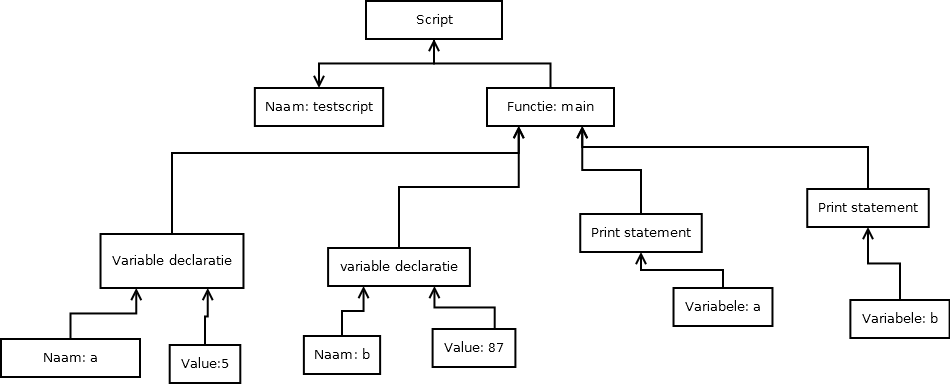
\includegraphics[width=\textwidth]{afbeeldingen/testsmall_tree}
\caption{Een voorbeeld van een syntaxboom}
\end{figure}

\subsection{Interpreter design pattern}
Het interpreter design pattern ligt aan de basis van onze interpreter. Dit design pattern zorgt ervoor dat we in staat zijn onze syntaxboom door te lopen en elke stap uit te voeren. Het hart van dit design pattern zit hem in de interpreter klasse. Deze klasse bevat een context object dat verantwoordelijk is voor het bijhouden van de symbolentabel en andere variabelen die belangrijk kunnen zijn voor de interpreter. Verder bevat de interpreter klasse ook nog een lijst met nodes. Deze nodes erven allemaal over van een gemeenschappelijke klasse die hen verplicht een interpret methode te implementeren. Deze methode voert de node uit en verandert, naargelang dit nodig is, de context van de interpreter. De execute methode van de interpreter zorgt ervoor dat de lijst van nodes die de interpreter bezit, overlopen wordt en er van iedere node de interpret methode wordt uitgevoerd.

\begin{figure}[ht]
\centering
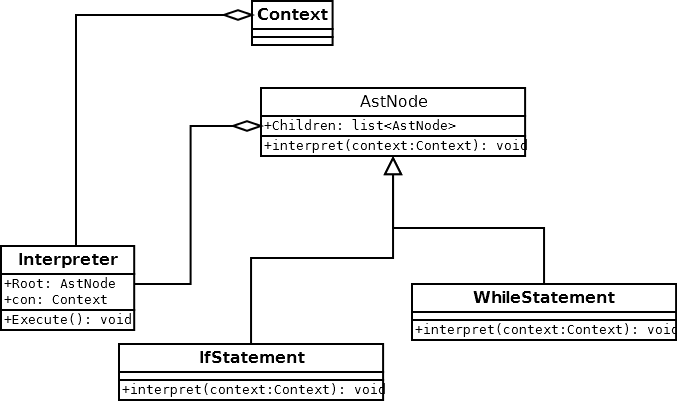
\includegraphics[width=\textwidth]{afbeeldingen/interpreter_small}
\caption{Het interpreter design pattern}
\end{figure}

\end{document}
